\documentclass[11pt,a4paper]{article}

\usepackage[
    a4paper,
    left=15mm,
    right=15mm,
    top=30mm,
    bottom=25mm,
    headheight=25mm
]{geometry}
\usepackage{graphicx}
\usepackage{polski}
\usepackage[utf8]{inputenc}
\usepackage{enumerate}
\usepackage{comment}
\usepackage{fancyhdr}
\usepackage{hyperref}
\usepackage{indentfirst}
\usepackage{multirow}
\usepackage{multicol}
\usepackage{float}
\usepackage{amsmath}
\usepackage{fancyhdr}
\usepackage{wrapfig}
\usepackage{layout}
\usepackage{textcomp}
\usepackage[center]{caption}
\usepackage{subcaption}
\usepackage{siunitx}
\usepackage[mathscr]{euscript}

\title{
    
\includegraphics[scale=0.42]{./res/logos/agh_logo_text_sym.jpg}
    \vfill
    Lokalizacja punktów w przestrzeni
    metodą trapezową.
}
\author{Łukasz Dragon, Rafał Babski}
\date{Algorytmy Geometryczne 2024/2025, grupa 1}

\sisetup{output-exponent-marker=\ensuremath{\mathrm{e}}}

\renewcommand{\baselinestretch}{1.18}
\renewcommand\thesubfigure{\roman{subfigure}}

\pagestyle{fancy}
\fancyhead[L]{
    
\includegraphics[scale=0.16]{./res/logos/agh_logo_text_asym.jpg}
}
\fancyhead[R]{
    Lokalizacja punktów w przestrzeni dwuwymiarowej metodą trapezową
    \\
    Łukasz Dragon, Rafał Babski
}

\begin{document}

\maketitle
\tableofcontents
\pagebreak

\section{Wstęp}

Celem projektu była implementacja algorytmu rozwiązującego
problem lokalizacji punktu w przestrzeni dwuwymiarowej 
metodą trapezową. W \hyperlink{section.2}{sekcji 2} znajduje się opis teoretyczny
działania algorytmu, wizualizacja wyników na zbiorach testowych
oraz analiza efektywności działania algorytmu. 
\hyperlink{section.3}{Sekcja 3} zawiera dokumentację załączonego w projekcie programu.

\section{Sprawozdanie}

\subsection{Wstęp teoretyczny}

\subsubsection{Opis problemu}
Problem lokalizacji punktu w przestrzeni dwuwymiarowej
można sformułować następująco:

Niech $\mathscr{S}$ oznacza podział przestrzeni dwuwymiarowej
zawierający $n$ krawędzi. Zapytanie o lokalizację punktu w $\mathscr{S}$
oznacza znalezienie takiej ściany $f$ zawartej w $\mathscr{S}$,
w której znajduje się zadany punkt $q$. Celem algorytmu jest
stworzenie takiej reprezentacji $\mathscr{S}$, która pozwala
odpowiadać na zapytanie lokalizacji punktu w jak najmniejszym
czasie. Stworzona przez nas reprezentacja powinna także 
zajmować jak najmniej miejsca w pamięci.

\subsubsection{Podział trapezowy}
Metoda trapezowa, nazywana także podziałem trapezowym,
polega na stworzeniu mapy trapezowej $\mathscr{T}(S)$
dla danego zbioru $S$ zawierającego $n$ odcinków, który
reprezentuje podział przestrzeni. Oprócz mapy $\mathscr{T}(S)$,
algorytm tworzy strukturę $\mathscr{D}$ pozwalającą odpowiadać
na zapytania lokalizacji punktu. Mapa trapezowa $\mathscr{T}(S)$
budowana jest w sposób przyrostowy poprzez dodawanie
kolejnych odcinków z $S$ i tworzenie pionowych przedłużeń wychodzących 
z ich wierzchołków i kończących się po napotkaniu innego odcinka.
Kolejność dodawania odcinków z $S$ wpływa na wielkość 
i czas odpowiedzi na zapytania struktury $\mathscr{D}$, 
jednak przy użyciu metody randomizacji, jesteśmy w stanie 
założyć \cite[s. 133-136]{compgeo}, że złożoność pamięciowa 
struktury $\mathscr{D}$ jest rzędu $O(n)$, a czas odpowiedzi 
na zapytanie rzędu $O(logn)$.
Ostatecznie, randomizowany algorytm przyrostowy budujący mapę
$\mathscr{T}(S)$ i strukturę $\mathscr{D}$ ma oczekiwaną 
złożoność obliczeniową $O(nlogn)$.

Podział trapezowy przyjmuje następujące założenia dla
zbioru $S$:
\begin{enumerate}
    \item Odcinki nie przecinają się.
    \item Wierzchołki odcinków mają parami różne współrzędne $x$.
\end{enumerate}

Zbiór $S$ spełniający powyższe założenia jest w \textit{położeniu ogólnym}.

Jesteśmy w stanie pozbyć się założenia 2 poprzez dokonanie
\textit{przekształcenia ścinającego} na odcinkach z $S$
o dostatecznie mały kąt $\varphi$ i stworzenie mapy trapezowej
dla nowo powstałego zbioru $\varphi S$, który już jest 
w \textit{położeniu ogólnym}.
Okazuje się jednak \cite[s. 137-139]{compgeo},
że przekształcenie to może pozostać jedynie w domyśle i
przy sprawdzaniu czy dany punkt leży na lewo od drugiego
wystaczy porównywać je leksykograficznie.

\subsubsection{Struktura mapy trapezowej}
Mapa trapezowa $\mathscr{T}(S)$ reprezentowana 
jest jako graf trapezów. Każdy stworzony trapez 
ma dwa boki pionowe (uznajemy także boki o długości zerowej).
Uznajemy, że dwa trapezy ze sobą sąsiadują gdy 
posiadają wspólną pionową ścianę. Dla zbioru
$S$ w \textit{położeniu ogólnym}, każdy trapez
ma maksymalnie czterech sąsiadów, do których
przechowujemy wskaźniki. Każdy trapez zawiera
także wskaźnik do odpowiadającego mu węzła
w strukturze przeszukiwań $\mathscr{D}$.

\subsubsection{Struktura przeszukiwań}
Struktura przeszukiwań $\mathscr{D}$ reprezentowana
jest przez \textit{acykliczny graf skierowany} 
przypominający strukturą drzewo binarne. Struktura
ta zawiera trzy typy węzłów:
\begin{enumerate}
    \item Węzeł trapezu
    - zawiera wskaźnik do trapezu w mapie $\mathscr{T}(S)$
    \item Węzeł wierzchołka
    - zawiera wskaźnik do jednego z wierzchołków odcinków z $S$
    oraz wskaźniki do dwóch węzłów-dzieci (lewego i prawego).
    \item Węzeł odcinka
    - zawiera jeden z odcinków z $S$
    oraz wskaźniki do dwóch węzłów-dzieci (lewego i prawego).
\end{enumerate}
Zapytanie w strukturze przechodzi następująco:

Zaczynamy w korzeniu grafu, w każdym węźle wierzchołka 
testujemy czy zadany punkt leży na lewo czy na prawo od 
trzymanego wierzchołka; jeżeli leży na prawo, to idziemy
do lewego dziecka, a w przeciwnym przypadku idziemy do prawego.
Analogicznie postępujemy w węzłach odcinka, tym razem jednak
testując czy zadany punkt leży nad odcinkiem (idziemy w lewo),
czy pod (idziemy w prawo). Jeżeli zadany punkt jest równy
jednemu z wierzchołków, bądź leży na jednym z odcinków, to
zwracamy odpowiednią informację.

\subsubsection{Opis algorytmu}
Algorytm w $i$-tym kroku buduje mapę $\mathscr{T}(S_i)$
oraz strukturę $\mathscr{D}_i$ dla listy punktów 
$S_i = (s_1, s_2, ..., s_i)$. Wynikiem jest mapa 
$\mathscr{T}(S_n)$ oraz struktura $\mathscr{D}_n$,
które zawierają wszystkie odcinki z $S$.
Poszczególne kroki algorytmu przebiegają następująco:
\begin{enumerate}
    \item Tworzymy prostokąt (trapez), w którym zawiera się
    każdy odcinek w $S$ i za jego pomocą inicjalizujemy
    strukturę $\mathscr{T}(S_0) := \mathscr{T}(\emptyset)$.
    \item Tworzymy listę $S_n = (s_1, s_2, ..., s_n)$ bedącą
    losową permutacją odcinków ze zbioru $S$.
    \item Dla każdego $i = 1, 2, ..., n$ powtarzamy:
    \begin{enumerate}
        \item Znajdujemy w obecnej mapie $\mathscr{T}(S_{i - 1})$
        trapezy $\Delta_1, \Delta_2, ..., \Delta_k$ przecięte
        przez odcinek $s_i$ (przecięcie tylko na wierzchołkach
        nie jest liczone).
        \item Usuwamy z $\mathscr{T}(S_{i - 1})$ trapezy
        $\Delta_1, \Delta_2, ..., \Delta_k$ zamieniając je
        na trapezy powstałe po dodaniu $s_i$. Otrzymujemy
        w ten sposób mapę $\mathscr{T}(S_i)$
        \item Usuwamy z $\mathscr{D}_{i - 1}$ węzły odpowiadające
        trapezom $\Delta_1, \Delta_2, ..., \Delta_k$
        i dodajemy węzły dla nowych trapezów odpowiednio
        je łącząc za pomocą węzłów wierzchołków i odcinków.
    \end{enumerate}
    \item Zwracamy $\mathscr{T}(S_n)$ jako wynik.
\end{enumerate}

Krok 3.(a) jesteśmy w stanie wykonać wykorzystując 
połączenia sąsiedzkie trapezów w mapie. Najpierw znajdujemy
trapez $\Delta_1$, wykonując zapytanie w strukturze $\mathscr{D}_{i - 1}$
dla punktu będącego lewym wierzchołkiem odcinka $s_i$.
Następnie podążamy wzdłuż odcinka $s_i$ przechodząc po i dodając do
listy przeciętych trapezów odpowiednich sąsiadów w mapie. Kończymy
po napotkaniu prawego wierzchołka odcinka $s_i$.
Dokładna implementacja wszystkich kroków algorytmu
znajduje się w załączonym programie opisanym 
w \hyperlink{section.3}{sekcji 3}. Opis każdego 
poszczególnego kroku algorytmu można znaleźć także
w: \cite[s. 129-133]{compgeo}

\subsection{Specyfikacja środowiska użytego do obliczeń}
Wyniki pokazane w sprawozdaniu zostały wygenerowane przy
użyciu interpretera języka Python wersji 3.9. Losowe 
zbiory odcinków przygotowane zostały przy pomocy biblioteki
\verb|numpy|. Wykresy i wizualizacja stworzonych przez
algorytm podziałów trapezowych została przygotowana za
pomocą narzędzia przygotowanego przez koło naukowe Bit,
dostępnego pod adresem: 
\emph{\hyperlink{https://github.com/aghbit/Algorytmy-Geometryczne}
{https://github.com/aghbit/Algorytmy-Geometryczne}}
Do przygotowania interaktywnego interfejsu pozwalającego
na zadawanie własnych zbiorów odcinków użyta została
biblioteka \verb|matplotlib|.
Wyniki przedstawione w tabelach: TODO: zostały wygenerowane
na komputerze z systemem operacyjnym Debian 12 i procesorem
AMD Ryzen 5 3600 3.6GHz.

\subsection{Testy i wizualizacja}
Przygotowaliśmy cztery zbiory odcinków w celu sprawdzenia
poprawności i wizualizacji działania algorytmu. Zbiory te
przedstawione są na rysunku 1. Rysunki 2, 3, 4, 5 zawierają
wizualizację map trapezowych wygenerowanych przez algorytm
kolejno dla zbiorów: A, B, C i D. Sekcje od 2.3.1 do 2.3.4 % TODO: Links?
zawierają także krótki komentarz na temat poszczególnych
zbiorów.

Animacje krokowe budowy mapy dla wspomnianych zbiorów
dostępne są do wygenerowania w pliku \textit{notatnika Python}
\verb|point_location.ipynb| (w tym celu należy zapoznać się
z dokumentacją w \hyperlink{section.3}{sekcji 3}).
Ponadto, wspomniane animacje zawarte są z projektem w formie
plików z rozszerzeniem \verb|gif|. Pliki te mają nazwy:
\verb|test_a_map.gif|, \verb|test_b_map.gif|,
\verb|test_c_map.gif|, \verb|test_d_map.gif|
i odpowiadają one kolejno zbiorom: A, B, C, D.

Animacje dla zbiorów zadanych przez użytkownika
dostępne są do wygenerowania w pliku: \\\verb|point_location.ipynb|.

\begin{figure}[H]
    \centering
    \begin{subfigure}[b]{0.46\textwidth}
        \centering
        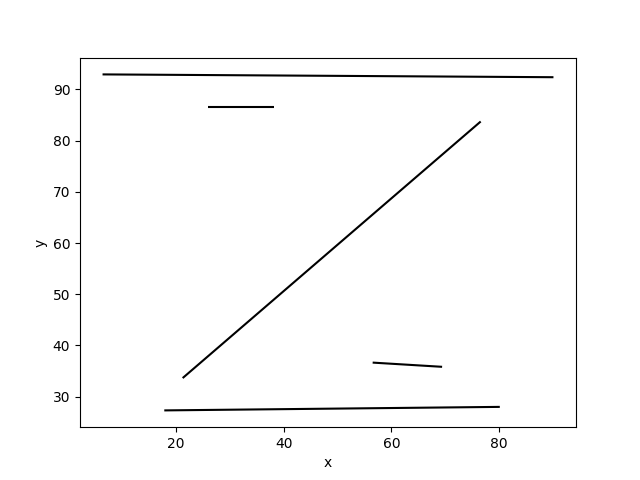
\includegraphics[scale=0.4]{res/figs/test_a.png}
        \caption{
            Zbiór A
        }
    \end{subfigure}
    \begin{subfigure}[b]{0.46\textwidth}
        \centering
        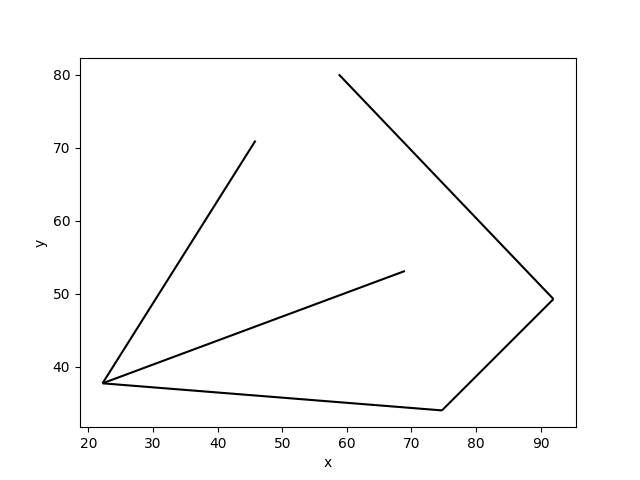
\includegraphics[scale=0.4]{res/figs/test_b.png}
        \caption{
            Zbiór B
        }
    \end{subfigure}
    \begin{subfigure}[b]{0.46\textwidth}
        \centering
        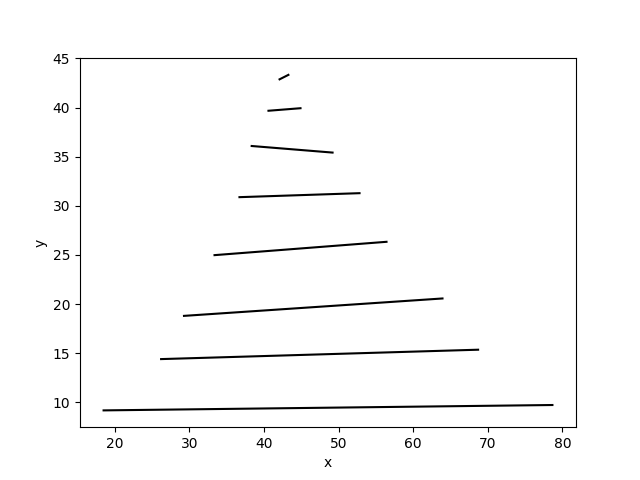
\includegraphics[scale=0.4]{res/figs/test_c.png}
        \caption{
            Zbiór C
        }
    \end{subfigure}
    \begin{subfigure}[b]{0.46\textwidth}
        \centering
        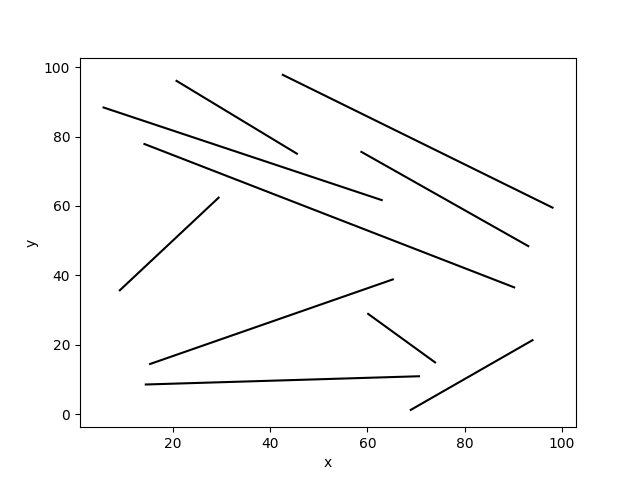
\includegraphics[scale=0.4]{res/figs/test_d.png}
        \caption{
            Zbiór D
        }
    \end{subfigure}
    \caption{Wybrane zbiory testowe}
\end{figure}

\subsubsection{Zbiór A}
Zbiór ten został przygotwany w celu sprawdzenia
czy algorytm poprawnie tworzy i scala trapezy.
Rysunek 2 zawiera wizualizację wygenerowanej mapy.

\begin{figure}[H]
    \centering
    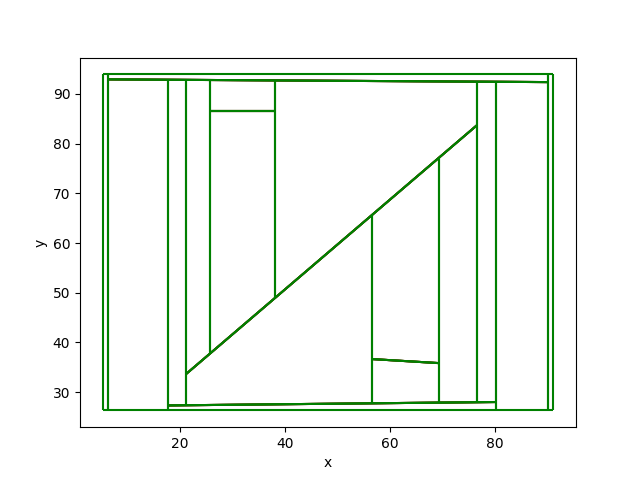
\includegraphics[scale=0.46]{./res/figs/test_a_map.png}
    \caption{Mapa trapezowa wygenerowana dla zbioru A}
\end{figure}

\pagebreak

\subsubsection{Zbiór B}
Zbiór ten został przygotowany w celu sprawdzenia
czy algorytm poprawnie radzi sobie w przypadku,
gdy odcinki łączą się w jednym punkcie. Rysunek 3
zawiera wizualizację wygenerowanej mapy.

\begin{figure}[H]
    \centering
    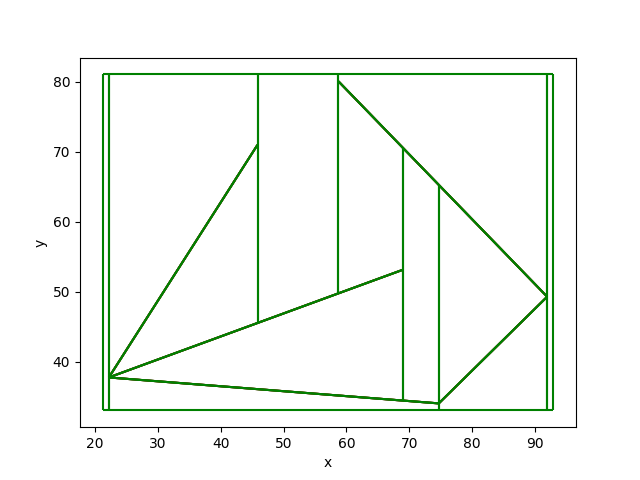
\includegraphics[scale=0.46]{./res/figs/test_b_map.png}
    \caption{Mapa trapezowa wygenerowana dla zbioru B}
\end{figure}

\subsubsection{Zbiór C}
Zbiór ten został przygotowany w celu sprawdzenia
czy algorytm poprawnie tworzy trapezy gdy każdy
odcinek zawiera się całkowicie wewnątrz jednego
trapezu. Rysunek 4 zawiera wizualizację wygenerowanej mapy.

\begin{figure}[H]
    \centering
    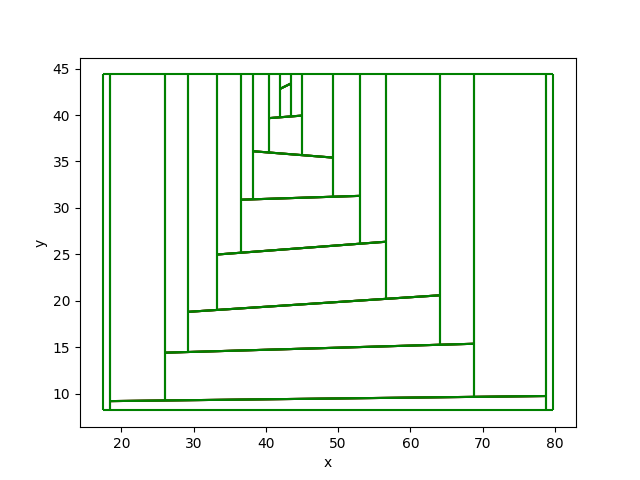
\includegraphics[scale=0.46]{./res/figs/test_c_map.png}
    \caption{Mapa trapezowa wygenerowana dla zbioru C}
\end{figure}

\pagebreak

\subsubsection{Zbiór D}
Zbiór ten został wygenerowany losowo i sprawdza
zarówno przypadki, w których odcinki zawierają się
w jednym trapezie, jak i w wielu. Rysunek 5
zawiera wizualizację wygenerowanej mapy.

\begin{figure}[H]
    \centering
    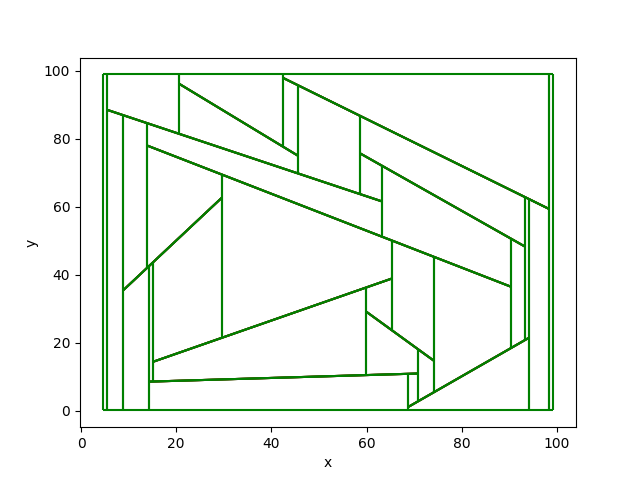
\includegraphics[scale=0.5]{./res/figs/test_d_map.png}
    \caption{Mapa trapezowa wygenerowana dla zbioru D}
\end{figure}

\subsection{Analiza efektywności algorytmu}
W celu analizy efektywności napisanego przez nas programu
przygotowaliśmy funkcję generującą losowy zbiór 
poziomych odcinków. Na tak przygotowanych zbiorach,
dla różnych liczb odcinków $n$, zmierzyliśmy średni
czas budowy mapy trapezowej przy pięciu wywołaniach.
Oprócz tego zliczyliśmy liczbę węzłów w wygenerowanych
strukturach przeszukiwań w celu oszacowania złożoności
pamięciowej programu (tutaj brane pod uwagę było jedno wywołanie). 
Ostatecznie, zmierzyliśmy średni czas
wykonania zapytania lokalizacji punktu w wygenerowanych
mapach dla 10000 losowo wygenerowanych punktów.

Tabela 1 zawiera wszystkie pomiary dla poszczególnych
wartości $n$. Rysunki 6, 7, 8 zawierają wykresy
poszczególnych zależności z tabeli 1 przyrównane do wykresów
funkcji rzędu oczekiwanych złożoności, czyli:
\begin{itemize}
    \item Rysunek 6 
    - Zależność czasu wykonania budowy mapy od $n$. 
    Oczekiwana złożoność $O(nlogn)$
    \item Rysunek 7
    - Zależność wielkości grafu przeszukiwań od $n$. 
    Oczekiwana złożoność $O(n)$
    \item Rysunek 8 
    - Zależność czasu wykonania zapytania lokalizacji punktu od $n$. 
    Oczekiwana złożoność $O(logn)$
\end{itemize}

\begin{table}[H]
    \centering
    \begin{tabular}{|r|r|r|r|}
    \hline
        $n$ & Średni czas budowy mapy [\si{s}] & Liczba węzłów w mapie & Średni czas zapytania [\si{s}]\\ \hline
        10 & 0,0023 & 81 & 0,000005872006416 \\ \hline
        50 & 0,0090 & 453 & 0,000007902321815 \\ \hline
        100 & 0,0111 & 928 & 0,000008317356110 \\ \hline
        500 & 0,0654 & 4930 & 0,000010902709960 \\ \hline
        1000 & 0,1456 & 9792 & 0,000011252136230 \\ \hline
        5000 & 0,8821 & 49847 & 0,000015353059770 \\ \hline
        10000 & 2,0014 & 99802 & 0,000016459221840 \\ \hline
        50000 & 11,4103 & 500394 & 0,000020709886550 \\ \hline
        100000 & 25,3333 & 1001918 & 0,000023330583570 \\ \hline
        500000 & 144,9936 & 4995205 & 0,000027396416660 \\ \hline
        1000000 & 319,7159 & 10003877 & 0,000031653146740 \\ \hline
    \end{tabular}
    \caption{Zależności czasu budowy mapy, jej wielkości 
    oraz czasu zapytania dla różnych wartości $n$.}
\end{table}

\begin{figure}[H]
    \centering
    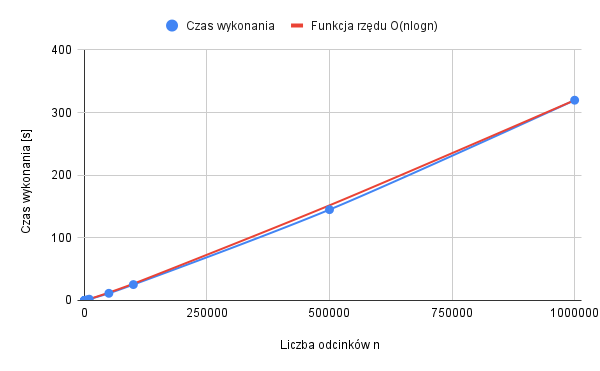
\includegraphics[scale=0.46]{./res/figs/build_times_graph.png}
    \caption{Zależność czasu wykonania budowy mapy od $n$.}
\end{figure}

\begin{figure}[H]
    \centering
    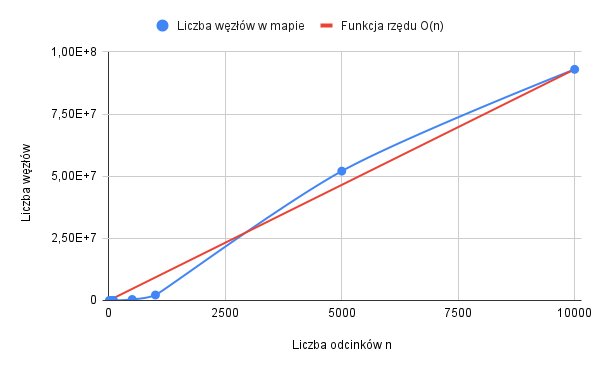
\includegraphics[scale=0.46]{./res/figs/build_sizes_graph.png}
    \caption{Zależność wielkości grafu przeszukiwań od $n$.}
\end{figure}

\begin{figure}[H]
    \centering
    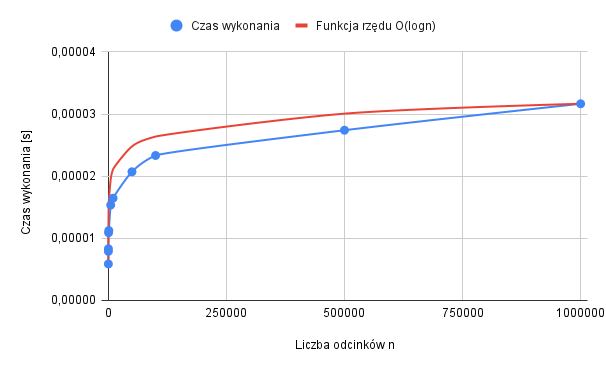
\includegraphics[scale=0.46]{./res/figs/query_times_graph.png}
    \caption{Zależność czasu wykonania zapytania lokalizacji punktu od $n$.}
\end{figure}

Jak możemy zauważyć na rysunkach 6, 7, 8, oczekiwana złożoność
czasowa i pamięciowa algorytmu budowy mapy oraz czasu zapytania
pokrywa się ze zmierzonymi przez nas wartościami.

\section{Dokumentacja}

Program napisany w ramach projektu podzielony jest
na dwa pliki: \verb|point_location.ipynb| \\
oraz \verb|creator.py|. Pierwszy z nich jest plikiem
\textit{notatnika Python} przygotowanym w celach dydaktycznych
dla użytkownika. Zawiera implementację, wizualizację na przykładach 
oraz możliwość testowania algorytmu na przygotowanych interaktywnie
zbiorach odcinków. Drugi jest natomiast plikiem
zawierającym kod realizujący interfejs graficzny dostępny w notatniku.

Sekcja 3.1 zawiera instrukcje potrzebne do wykonania programu,
sekcja 3.2 zawiera dokumentację skierowaną do użytkownika, %TODO: Links?
a sekcja 3.3 opisuje dokładnie najważniejsze funkcje, metody
i obiekty stworzone w celu implementacji algorytmu.

\subsection{Instrukcja wykonania programu}
Notatnik \verb|point_location.ipynb| należy wykonać
wewnątrz środowiska dostępnego w narzędziu 
przygotowanym przez studentów z koła naukowego Bit, 
które jest dostępne pod adresem:
\\
\emph{\hyperlink{https://github.com/aghbit/Algorytmy-Geometryczne}
{https://github.com/aghbit/Algorytmy-Geometryczne}}
\\
Program należy wykonywać w ten sam sposób co
zawarte w narzędziu programy przygotowane na laboratoria.

\subsection{Część użytkownika}
W celu uruchomienia programu należy po kolei
wykonywać komórki wewnątrz notatnika \\
\verb|point_location.ipynb|. Plik ten zawiera
krótkie opisy problemu, algorytmu oraz zaimplementowanych
przez nas struktur. Oprócz tego nad każdą metodą i obiektem
znajdują się komentarze tłumaczące ich cel i działanie.

Pod nagłówkiem \emph{"Interaktywne zadawanie zbioru odcinków"}
znajduje się odpowiednio komórka, której wykonanie otworzy
okno pozwalające na interaktywne zadawanie zbioru odcinków.
Kliknięcie lewym przyciskiem myszy w dwóch miejscach stworzy odcinek. 
Program nie pozwoli na stworzenie odcinka przecinającego się z innym.
Przycisk \emph{"Wyczyść"} usuwa wszystkie stworzone odcinki.
Odcinki można zapisać do pliku o formacie \verb|json| po kliknięciu
przycisku \emph{"Zapisz"}. Alternatywnie do zadawania odcinków myszką,
możliwe jest wygenerowanie zbioru odcinków losowo po wciśnięciu
przycisku \emph{"Wygeneruj losowo odcinki"}, wpisaniu interesujących
nas parametrów i zatwierdzeniu przyciskiem \emph{"OK"}. Zamknięcie
okna możliwe jest przy pomocy przycisku \emph{"OK"}.

Po wygenerowaniu zbioru odcinków, wywołanie kolejnej komórki
wypisze na ekran ich współrzędne oraz wyświetli krokową
wizualizację budowy mapy trapezowej na zadanym przez użytkownika
zbiorze.

Następne komórki zawierają kod generujący animacje krokowe
dla wybranych zbiorów testowych oraz dane potrzebne do
analizy efektywności algorytmu.

\subsection{Część techniczna}
Algorytm budujący podział trapezowy dla zadanego
zbioru odcinków skupiony jest wewnątrz funkcji
\verb|build_trapezoidal_map|. Funkcja ta zwraca
obiekt \verb|TrapezoidalMap|, który zawiera w sobie
zarówno reprezentację mapy trapezowej, jak 
i graf przeszukiwań. Dokładne kroki budowy 
znajdują się wewnątrz metod obiektu \verb|TrapezoidalMap|.
Oprócz obiektu mapy istnieją także następujące obiekty
pomocnicze:
\begin{itemize}
    \item \verb|Trapezoid| - reprezentuje pojedynczy trapez, 
    zawiera indeksy odcinków definiujących go z góry i z dołu 
    (\verb|top| i \verb|bottom|) oraz indeksy wierzchołków
    definiujących go z lewej i z prawej (\verb|leftp|, \verb|rightp|).
    Metoda \verb|as_verticies| pozwala obliczyć dokładne współrzędne
    wierzchołków trapezu.
    \item \verb|TrapezoidNode| - reprezentuje węzeł trapezu
    w grafie przeszukiwań. Zawiera wskaźniki do odpowiadającego
    mu obiektu \verb|Trapezoid| oraz do wszystkich z jego
    maksymalnie czterech sąsiadów (\verb|left_lower|, \verb|left_upper|, 
    \verb|right_lower|, \verb|right_upper|). Posiada także wskaźniki
    do własnych przodków w grafie.
    \item \verb|XNode| - reprezentuje węzeł wierzchołka. Zawiera
    indeks odpowiadającego mu punktu (\verb|x|) oraz
    wskaźniki do lewego i prawego dziecka (\verb|left| i \verb|right|).
    \item \verb|YNode| - reprezentuje węzeł odcinka. Zawiera
    indeks odpowiadającego mu odcinka (\verb|edge|) oraz
    wskaźniki do lewego i prawego dziecka (\verb|left| i \verb|right|).
\end{itemize}
Wszystkie obiekty typu \verb|Node| posiadają metodę \verb|follow|,
która przyjmuje punkt i zwraca wskaźnik do dziecka, do którego
powinniśmy dalej przejść. \verb|XNode| prowadzi do lewego
dziecka gdy dany punkt leży po lewej od trzymanego wierzchołka
i do prawego gdy leży po prawej. \verb|YNode| prowadzi do lewego
dziecka gdy punkt leży ponad trzymanym odcinkiem i do prawego
gdy leży pod. Jeżeli punkt znajduje się wewnątrz węzła
(jest wewnątrz trapezu, jest już wierzchołkiem, bądź leży na odcinku)
zwracana jest wartość \verb|None|.

Obiekt \verb|TrapezoidalMap| zawiera w sobie wskaźnik do
węzła korzenia (\verb|root|), indeks ostatnio dodanego wierzchołka
oraz wskaźnik do listy odcinków (\verb|sections|). Inicjalizując
obiekt tworzymy mapę zawierającą tylko jeden trapez - prostokąt,
otaczający wszystkie odcinki.

Opiszemy teraz najważniejsze metody obiektu \verb|TrapezoidalMap|:
\begin{itemize}
    \item \verb|advance_i| - dodaje kolejny odcinek z podanej 
    listy do mapy, aktualizując wewnętrzną strukturę tak, aby
    reprezentowała graf przeszukiwań i mapę trapezową uwzględniającą
    nowo dodany odcinek.
    \item \verb|find_section_zone| - zwraca listę trapezów
    przeciętych przez podany odcinek.
    \item \verb|partition_zone| - dzieli wszystkie trapezy
    przecinane przez dany odcinek na mniejsze, aktualizując
    sąsiedztwa i strukturę grafu przeszukiwań. Dzieli się 
    na cztery przypadki rozważane w następujących metodach:
    \begin{enumerate}
        \item \verb|partition_one| - odcinek przecina dokładnie
        jeden trapez i znajduje się całkowicie wewnątrz niego.
        Zawsze tworzy cztery trapezy.
        \item \verb|partition_one_tri_left| i \verb|partition_one_tri_right| -
        przypadki symetryczne: odcinek przecina dokładnie jeden trapez,
        lecz jeden z jego wierzchołków (lewy lub prawy) znajduje się już
        w mapie. Zawsze tworzy trzy trapezy.
        \item \verb|partition_multi| - odcinek przecina więcej niż jeden
        trapez. Algorytm idzie wzdłuż odcinka, usuwając stare trapezy
        i tworząc nowe, łącząc niektóre z nich w jeden.
    \end{enumerate}
    \item \verb|find| - zwraca węzeł w grafie przeszukiwań
    zawierający dany punkt.
    \item \verb|find_trapezoid| - działa analogicznie do \verb|find|,
    lecz zawsze zwraca trapez. Gdy punkt jest już wierzchołkiem,
    przyjmujemy, że leży on po prawo, a gdy leży na odcinku, to uznajemy,
    że leży nad nim.
    \item \verb|get_trapezoids| - zwraca listę trapezów wewnątrz mapy.

W celu wizualizacji kroków algorytmu stworzona została także
metoda: \\ 
\verb|build_trapezoidal_map_visualization| korzystająca 
z narzędzia do wizualizacji przygotowanego przez koło naukowe Bit.
\end{itemize}

\section{Podsumowanie}
W ramach projektu zaimplementowaliśmy algorytm lokalizacji
punktu w przestrzeni metodą trapezową. Zaimplementowana przez
nas funkcja budująca graf przeszukiwań i mapę trapezową przeszła
wszystkie testy, pokrywając się po wizualizacji z naszymi oczekiwaniami.
Przygotowaliśmy także animacje krokowe pokazujące działanie algorytmu,
które poza wsparciem nas w wykrywaniu błędów na etapie pisania kodu,
pokazują jasno kolejne kroki algorytmu. Animacje dla zbiorów testowych dołączone 
są razem z projektem w postaci plików: \verb|test_a_map.gif|, 
\verb|test_b_map.gif|, \verb|test_c_map.gif| oraz \verb|test_d_map.gif|.
Zaimplementowany został także interfejs pozwalający użytkownikowi na
zadawanie własnych zbiorów odcinków i pokazujący zbudowaną dla nich
mapę trapezową. Ostatecznie zmierzyliśmy czas wykonania budowy mapy,
jej wielkość oraz czas wykonania zapytania lokalizacji punktu dla różnych
liczb odcinków w zbiorze wejściowym. Wykresy zmierzonych wartości
pokrywają się z wykresami oczekiwanych złożoności pamięciowych i obliczeniowych
algorytmu.

\begin{thebibliography}{999}
\bibitem{compgeo}
    M. van de Berg, M. van Kreveld, M. Overmars, and O. Schwarzkopf,
    (1997)
    \emph{Computational Geometry},
    Springer.
\end{thebibliography}

\end{document}